\section{Homework 1}
\begin{problem} Foiling Cryptanalsis. \end{problem}
\solution Text text text.

\section{Homework 2}

\section{Homework 3}
\begin{problem} Encode the message "CATSRCOOL" as an integer that someone in Monday's class would know how to decode (s=3).
\solution Since $s=3$, break into three letter intervals: $$CAT|SRC|OOL.$$ Now, take each 3-letter string and take it as a base-26 number, and convert to base-10. $$(CAT)_
{26} = 2(26)^2 + 0(26)^1 + 19 (26)^0 = 1371.$$
Knowing s=3, we know the longest possible number has 5 digits so add a zero to begin the number. Thus, $$(CAT)_{26}=01371.$$
$$(SRC)_{26} = 18(26)^2 + 17(26)^1 + 2(26)^0=12612$$ $$(OOL)_(26) = 14(26)^2 + 14(26)^1 + 11(26)^0 = 09839.$$ Therefore, CATSRCOOL would be encoded as 013711261209839.

\begin{problem} Decode 044340261411777 (encoded with $s=3$). Note any nulls at the end of the message and discard.
\end{problem}
\solution Since $s=3$, we know the largest possible number ($26^3-1=17575$) has five digits, so we break the message into 5 digit intervals: $$04434|02614|11777.$$ Now, convert each string from base-10 to base-26. $$04434=4434=170(26)+14=6(26)^2 +14(26)^1 + 14 = (GOO)_{26}$$ $$02614=2614=100(26)+14(26)^0 = 3(26)^2 + 22(26)^1 + 14(26)^0 = (DWO)_{26}$$ $$11777=452(26) + 25 = 17(26)^2 + 10(26)^1 + 25 (26)^0 = (RKZ)_{26}.$$ Dismishing Z as a null, we decode 044340261411777 as GOODWORK.
\section{Homework 4}
\begin{problem}  Without converting to base-17, find an expression for the number of digits that the integer
$13,335,689,990,113,121$ will have in base-17. Use a calculator or computer to determine the exact
answer.
\end{problem}
\solution 
Let $n = 13,335,689,990,113,121, b = 17$. 
Then, the number of digits of the integer $n$ in base-17, $k = [\frac{ln(n)}{ln(b)}] + 1 = 13 + 1 = 14$. 
\begin{problem}
 Find all the divisors of $8^{10} - 1$ of the form $2n - 1$ where $2 \leq n$.
\end{problem}
\solution 
$8^{10}-1 = (2^{3})^{10}-1 = 2^{3*10} - 1 = 2^{2*15} - 1 = 2^{5*6} - 1 = 2^{1*30}-1$
By the corollary that $b^{mn}-1 = (b^{m}-1)(b^{m(n-1)} + b^{m(n-2)} + .....+ b^{m} +1)$, $8^{10} - 1$ is divisible by $2^{2}-1, 2^{3}-1, 2^{5}-1, 2^{6}-1, 2^{10}-1, 2^{15}-1$, and $2^{30}-1$.
\begin{problem}
If $d$ divides $a$ and $b$, then $d$ divides $a - bq$ for any $q \in Z$.
\end{problem}
\solution
\begin{proof} 
Let $a,b,d \in \mathbb{Z}$ such that $d|a$ and $d|b$. Since $d|a, a = dm$ for some $m \in \mathbb{Z}$. Similarly, since $d|b, b = dn$ for some $n \in \mathbb{Z}$. Consider $a-bq$, where $q \in \mathbb{Z}$. By substitution, $a-bq=dm-dn(q)=dm-dnq$. By distributivity, $dm-dnq=d(m-nq)$. Since $a-bq=d(m-nq), d|a-bq$.
\end{proof}
\begin{problem} If $d$ divides $a-bq$, then $d$ divides $a$ and $b$.
\end{problem}
\solution
Counter example: Let $d=3,a=10,b=2,q=2$. $d|a-bq=6$. Then, $d$ divides $a-bq$, but d does not divide $a$ or $b$.
\begin{problem} If $d$ divides $ab$, then $d$ divides $a$ or $b$.
\end{problem}
\solution
Counter example: let $d=6,a=3,b=10$. Therefore, $d$ divides $ab$, but $d$ does not divide $a$ or $b$. 
\begin{problem} If $4$ divides $ab$, then $a$ or $b$ is even.
\end{problem}
\solution
\begin{proof}
Let $a,b \in \mathbb{Z}$ such that $4|ab$. 
Since $4|ab$, $2|ab$ and $ab$ is even. 
Suppose that $a,b$ are odd and $a=2n+1, b=2m+1$, where $m,n \in \mathbb{Z}$.Then, $ab=(2n+1)(2m+1)=4nm+2n+2m+1$,which clearly is odd. This is a contradiction to the fact that $ab$ is even.
Next, suppose that $a=2n$ is even and $b=2m+1$ is odd. Then, $ab=(2n)(2m+1)=4nm+2n$,which clearly is even.  
Therefore, if $4$ divdies $ab$,then $a$ or $b$ is even. 

\end{proof}
\begin{problem}If $6$ divides $ab$, then $a$ or $b$ is odd.
\end{problem}
\solution
Counter example: Let $a=b=6$. Then, $6$ divides $ab$, but $a$ and $b$ are even. 
\begin{problem}Find the greatest common divisor $d$ of each pair $a$ and $b$ below, and then find some $x$ and $y$ so that $d=ax+by$.\\
$(a)$ $a \in \mathbb{Z}$(any integer), $b=0$
\end{problem}
\solution 
$d=a$ because $0$ is divisible by any integer. 
Thus,$d=ax+by=a$ where $x=1$ and $y$ can be any integer. 
\begin{problem}
$(b)$ $a=105,b=17$
\end{problem}
\solution 
\\Using the division algorithm,
\\$105=17*6+3$
\\$17=3*5+2$
\\$3=2*1+1$
\\$2=1*2$ 
\\Thus, $d(105,17)=1$. 
\\Substituting back, 
\\$1=3-2*1=3-(17-3*5)*1=3*6-17= (105-17*6)*6-17=105*6-17*37$
\\Thus,$1=105*6+17*(-37)$where $x=6,y=37$.
\begin{problem}
$(c)$ $a = (KG)_{26}, b = (BA)_{26}$ ($d$ should be expressed in base-26, too)
\end{problem}
\solution
\\$a=(KG)_{26} = (10$ $6)_{26}=266, b=(BA)_{26} = (1$ $0)_{26}=26$. 
\\Using the division algorithm, 
\\$266=26*10+6
\\26=6*4+2
\\6=2*3$
\\Thus, $d(266,26)=2$. 
\\Substituting back, 
\\$2=26-6*4= 26-(266-26*10)*4 = 26-266*4+26*40=266*(-4) + 26*41$
\\Thus, $2=266*(-4)+26*41$, where $x=-4,y=41$. 
\\Therefore, $d=(C)_{26}=-4(KG)_{26}+(BA)_{26}(BP)_{26}$. 
\section{Homework 5}

\begin{problem}
Encipher the message "don’t forget to deflate the footballs" with the code word PATS.
\end{problem}

\solution
\begin{table}[!h]\label{tab:base26digits}
\centering
\begin{small}
\begin{tabular}{|c|c|c|c|c|c|c|c|c|c|c|c|c|}
\hline
a & b & c & d & e & f & g & h & i & j & k & l & m \\
\hline
P & Q & R & S & T & U & V & W & X & Y & Z & A & B \\
\hline
A & B & C & D & E & F & G & H & I & J & K & L & M \\
\hline
T & U & V & W & X & Y & Z & A & B & C & D & E & F \\
\hline
S & T & U & V & W & X & Y & Z & A & B & C & D & E \\
\hline
\multicolumn{13}{ c }{    } \\
\hline
n & o & p & q & r & s & t & u & v & w & x & y & z\\
\hline
C & D & E & F & G & H & I & J & K & L & M & N & O\\
\hline
N & O & P & Q & R & S & T & U & V & W & X & Y & Z \\
\hline
G & H & I & J & K & L & M & N & O & P & Q & R & S \\
\hline
F & G & H & I & J & K & L & M & N & O & P & Q & R \\
\hline
\end{tabular}
\caption{Enciphering with a Vigen\`{e}re Cipher (code word: PATS)}
\end{small}
\end{table}

Where $n \in \mathbb{Z}$, every 4n+1th letter will be enciphered with the row
that begins with P, every 4n+2th letter with the row that begins with A, every
4n+3rd letter with the row that begins with T, and every 4nth letter with the
row that begins with S. Thus,


plaintext  don't forget to deflate the footballs 


ciphertext SOG'L UOKYTT MG SEYDPTX LWE YGDTUSALL  


\begin{problem}
Crack the message VBX GCNL EPX MLG XHKU UGH VBX KKVUSPM.
\end{problem}
\solution Since there are 20 letters between the two occurrences of "VBX," the possible code word lengths are 1, 2, 4, 5, 20. If we guess that "VBX" is one of the most common three letter words in the English language, "the", then we create the following table:

\begin{table}[!h]\label{tab:base26digits}
\centering
\begin{small}
\begin{tabular}{|c|c|c|c|c|c|c|c|c|c|c|c|c|}

\hline
a & b & c & d & e & f & g & h & i & j & k & l & m \\
\hline
C & D & E & F & G & H & I & J & K & L & M & N & O  \\
\hline
U & V & W & X & Y & Z & A & B & C & D & E & F & G  \\
\hline
T & U & V & W & X & Y & Z & A & B & C & D & E & F \\
\hline
& & & & & & & & & & & &\\
\hline
\multicolumn{13}{ c }{    } \\
\hline
n & o & p & q & r & s & t & u & v & w & x & y & z\\
\hline
P & Q & R & S & T & U & V & W & X & Y & Z & A & B\\
\hline
H & I & J & K & L & M & N & O & P & Q & R & S & T \\
\hline
G & H & I & J & K & L & M & N & O & P & Q & R & S \\
\hline
& & & & & & & & & & & &\\
\hline

\end{tabular}
\caption{Enciphering with a Vigen\`{e}re Cipher (code word: CUT??)}
\end{small}
\end{table}

Since the code word is most likely 4 or 5 letters, I am going to guess that the code word is "CUTE."

\begin{table}[!h]\label{tab:base26digits}
\centering
\begin{small}
\begin{tabular}{|c|c|c|c|c|c|c|c|c|c|c|c|c|}

\hline
a & b & c & d & e & f & g & h & i & j & k & l & m \\
\hline
E & F & G & H & I & J & K & L & M & N & O & P & Q\\
\hline
\multicolumn{13}{ c }{    } \\
\hline
n & o & p & q & r & s & t & u & v & w & x & y & z\\
\hline
R & S & T & U & V & W & X & Y & Z & A & B & C & D\\
\hline

\end{tabular}
\caption{Enciphering with a Vigen\`{e}re Cipher (code word: CUTE)}
\end{small}
\end{table}

ciphertext VBX GCNL EPX MLG XHKU UGH VBX KKVUSPM


plaintext  the cats and the dogs and the gibbons


\begin{problem}
Describe one way to make a polyalphabetic cipher more secure than the Vigen\`{e}re cipher.
\end{problem}
\solution A polyalphabetic substitution cipher 


\begin{problem}
Find five distinct integer solutions to the equation 4x + 6y = 8 and make a
conjecture about how all integer solutions to this equation are related.
\end{problem}

\solution
Some solutions are..
($x=2$, $y=0$), ($x=5$, $y=-2$), ($x=8$, $y=-4$), ($x=11$, $y=-6$), ($x=14$, $y=-8$)

Conjecture: for all solutions, there exists $n \in \mathbb{Z}$ such that
$y=-2n$ and $x=2+3n$.

\section{Homework 6}

\begin{problem}[1] For all nonzero integers $a,b,c \in \mathbb Z$, the equation 
\begin{equation} \label{6.1}
ax + by + cz = n
\end{equation}
has an integer solution if and only if $n$ is a multiple of $d = \gcd(a,b,c)$.
\end{problem}
\begin{proof} $(\Longrightarrow)$ Suppose \ref{6.1} has an integer solution. Let $q_a, q_b, q_c \in \mathbb Z$ satisfy $dq_a = a$, $dq_b = b$, $dq_c = c$. Then if $x_0,y_0,z_0 \in \mathbb Z$ solve \ref{6.1}, we may rewrite the equation as
\[
n = dq_ax_0 + dq_by_0 + dq_cz_0 = d(q_ax_0 + q_by_0 + q_cz_0),
\]
and since $q_ax_0 + q_by_0 + q_cz_0 \in \mathbb Z$, this shows that $n$ is a multiple of $d$. 

$(\Longleftarrow)$ Now suppose that $d$ divides $n$. Let $d' := \gcd(a,b)$. Then since $d$ divides both $a$ and $b$, it follows that $d$ divides $d'$ by the definition of a greatest common divisor. By hypothesis, $d$ divides $c$ as well. Suppose $k \in \mathbb Z$ divides both $d'$ and $c$. Then since $k$ divides $d'$, $k$ must divide $a$ and $b$. Also, since $k$ divides $c$ as well, we must have that $k$ divides $d$, again by the definition of a greatest common divisor. Since $d$ divides both $d'$ and $c$, and since $k$ divides $d$ for any $k \in \mathbb Z$ dividing both $d'$ and $c$, we must have that
\begin{equation} \label{6.2}
d = \gcd(d',c) = \gcd(a,b,c).
\end{equation}
By the Euclidean Algorithm, there must exist $x', y' \in \mathbb Z$ for which
\begin{equation} \label{6.3}
ax' + by' = d',
\end{equation}
as well as $w',z' \in \mathbb Z$ for which 
\begin{equation} \label{6.4}
d'w' + cz' = d.
\end{equation}
Since $d$ divides $n$ by hypothesis, let $q \in \mathbb Z$ satisfy $dq = n$. Then \ref{6.4} becomes
\begin{equation} \label{6.5}
d'w'q + cz'q = dq = n.
\end{equation}
Substituting the lefthand side of \ref{6.3} in for $d'$ in \ref{6.5} gives us
\[
(ax' + by')w'q + cz'q = n,
\]
or equivalently, 
\[
\boxed{ a(x'w'q) + b(y'w'q) + c(z'q) = n } \,.
\]
Since $x'w'q$, $y'w'q$, and $z'q$ are all integers, we have an integer solution to \ref{6.1}.
\end{proof}

\begin{problem}[2] Let $m,n,p,q \in \mathbb Z$. Then the assigments $x=mn$, $y=pq$, $z=mp$, and $w=nq$ form an integer solution to the diophantine equation $xy=zw$. 
\end{problem}
\begin{proof} By commutativity and associativity of integer multiplication, we have: 
\[
xy = (mn)(pq) = m(np)q = m(pn)q = (mp)(nq) = zw,
\]
so $(x,y,z,w) = (mn,pq,mp,nq)$ is a solution. \end{proof}
\end{problem}

\begin{problem}[3] \ \\
\noindent (a) A number $N \in \mathbb Z$ is triangular if and only if there exists some $n \in \mathbb Z$ for which $N = \sum_{k=1}^n k$. 
\begin{proof} $(\Longrightarrow)$ Let $N \in \mathbb Z$ be triangular. Consider the triangular arrangement of $N$ balls. In any row $k$ of the triangle, each ball must have under it in row $k+1$ one ball on either side. For example, in the triangle of 28 balls shown below, each ball in row 4 has one ball on either side underneath it in row 5.
\begin{figure}
\centering
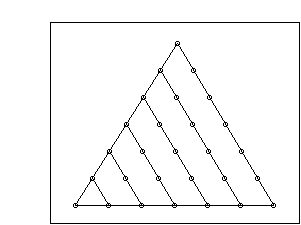
\includegraphics[scale=0.5]{triangular}
\caption{$T_7 = 28$}
\end{figure}
In order to accomplish this, we can begin from the left in each row, and add balls going right until the condition is satisfied in the row we're constructing. If $N$ is triangular, this process will result in a complete equilateral triangle. Each ball in a given row has one ball below and to the left (except the bottom row), and the ball furthest to the right has an additional ball below and to the right. So each row has exactly one more ball than the row above it. 

Suppose no $n \in \mathbb Z$ satisfies $N = \sum_{k=1}^n k$. Then some row will necessarily be incomplete once all $N$ balls have been placed, since otherwise $N = \sum_{k=1}^n k$ for some $n \in \mathbb Z$. This contradicts our hypothesis that $N$ is triangular. Therefore there must be some $n \in \mathbb Z$ for which $N = \sum_{k=1}^n k$. 

$(\Longleftarrow)$ Now suppose $N = \sum_{k=1}^n k$ for some $n \in \mathbb Z$. Then, 
\[
N = 1 + 2 + \cdots + n.
\]
Place $k$ balls in each row $k$, starting with $k=1$, and align each row below each previous row, where each successive row has one more ball. Stop at $k=n$. The resulting array of balls will be an equilateral triangle. If we add up the number of balls in each row, we get $1 + 2 + \cdots + n$, which by hypothesis is $N$. So $N$ is triangular. 
\end{proof}

\noindent (b) A number is triangular if and only if it is of the form $\frac{n(n+1)} 2$ for some $n \in \mathbb Z$. 
\begin{proof} $(\Longrightarrow)$ Suppose $N \in \mathbb Z$ is triangular. Then as we have shown, there exists some $n \in \mathbb Z$ so that 
\begin{equation} \label{6.6}
N = 1 + 2 + \cdots + n.
\end{equation}
By additive commutativity, this is equivalent to 
\begin{equation} \label{6.7}
N = n + (n-1) + \cdots + 2 + 1.
\end{equation}
Adding each term of \ref{6.6} and \ref{6.7} gives
\begin{align*}
2N &= (n+1) + (n-1 + 2) + \cdots + (2+n-1) + (1+n) \\
&= (n+1) + (n+1) + \cdots + (n+1) + (n+1) \\
&= n(n+1).
\end{align*}
Therefore $N = \frac{n(n+1)}2$. 

$(\Longleftarrow)$ Suppose $N = \frac{n(n+1)}2$ for some $n \in \mathbb Z$. Reversing the above algebraic steps gives
\[
2N = 2(1 + 2 + \cdots + n),
\]
so $N = 1 + 2 + \cdots + n$, and as we've shown, this implies that $N$ is triangular. \end{proof}

\noindent (c) The sum of any two consecutive triangular numbers is a perfect square. 
\begin{proof} Two consecutive triangular numbers must be of the form $\frac{n(n+1)}2$ and $\frac{(n+1)(n+2)}2$. Their sum is thus: 
\begin{align*}
\frac{n(n+1)}2 + \frac{(n+1)(n+2)}2 &= \frac{n^2 + n}2 + \frac{n^2 + 3n + 2}{2}\\
&= \frac{2n^2 + 4n + 2}2 \\
&= n^2 + 2n + 1 \\
&=(n+1)^2.
\end{align*} 
\end{proof}

\noindent (d) We will define a \emph{pentagonal number} as one that can represent the number of vertices in a pentagonal graph with equal vertices on each side, and successively smaller pentagonal subgraphs embedded in the original graph so that all subgraphs share one corner vertex. The first four pentagonal numbers are displayed below. 

\begin{figure}
\centering
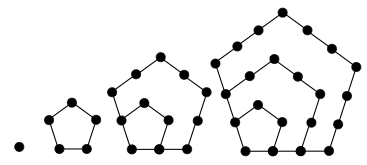
\includegraphics{pentagonal}
\caption{Pentagonal numbers}
\end{figure}

\end{problem}


\section{Homework 7}

\section{Homework 8}
\begin{problem}
A switchboard has ten cables that connect ten of the letters a through z to ten of the letters A through Z. How many ways are there to arrange the ten cables? For the purposes of this exercise,
note that $a\leftarrow B$ is different than $b\leftarrow A$.

\solution
The number of ways to choose 10 elements from $\{ a,. . ., z\}$ is 26 choose 10, i.e. ${26 \choose 10} = {\frac {26!}{16!10!}}= {5,311,735}$. Furthermore, the number of ways to choose 10 elements in $\{A,. . . , Z\}$, where order matters, is the number of permutations of 10 elements in a set of 26 elements: ${\frac {26!}{16!}}= {19,275,223,968,000}$. By multiplying these numbers we find that the number of ways to hook up the cables is $1.02384882*10^{20}$, or if you prefer, ${26 \choose 10}({\frac{26!}{16!}})$. 

\begin{problem}
I have three racks ($R_{1}$, $R_{2}$, and $R_{3}$), each of which holds 26 different hats. I’m planning on wearing
three hats today (it’s cold!), and I’m going to pick my first hat from $R_{1}$, my second hat from $R_{2}$,
and my third hat from $R_{3}$. How many ways can I wear my hats?

\solution
First, you have 26 different options. After making the first choice, there are 26 more options, so $26^{2}$. Finally, after making the second choice there are 26 more options for $R_{3}$. So $26^{3}$ is the number of options total.

\begin{problem}
It’s roughtly 50 years in the future. I’ve exhausted my hat combinations, and I want to mix things
up. If go truly crazy and pick my three daily hats from $R_{1}$, $R_{2}$, and $R_{3}$ in any order, how many
distinct hat combinations are possible? (Wearing hat A on top of hat B is different than wearing
hat B on top of hat A.)

\solution
There are $26^{3}$ different ways of choosing a hat from each rack (as shown by the previous problem). However, if the order of choosing the hats matters, there are more. Since each choice of 3 hats can be worn $3!=6$ different ways (which is the number of ways to permute the three hats), there are $6*26^{3}$ different options.


\section{Homework n+1}

\begin{problem}
Fill in the addition table below for the elliptic curve $E : y^2 = x^3 + 2x + 1$ over the finite field $\mathbb{F}_5$.

\solution
For points $(x_1, y_1)$ and $(x_2, y_2)$ on an elliptic curve $E= x^3 + ax + b$ over the finite field $\mathbb{F}_n$, If $x_1 = x_2$ and $y_1 \equiv -y_2$ (mod n), then $(x_1, y_1) + (x_2, y_2)$ = $\mathcal{O}$. Thus $(1,2) + (1,3) = (3,2) + (3,3) = (0,4) + (0,1) = \mathcal{O}$.

The equations to find $(x_1, y_1) + (x_2, y_2)  = (x_{3},y_{3})$ are as follows.
$$x_{3} = \lambda ^2 - x_{1} - x_{2}$$
$$y_{3}=\lambda(x_{1}-x_{3})-y_{1}$$

If $(x_1, y_1) = (x_2, y_2)$, then $ \lambda = (3x_{1}^2+A){(2y_{1})}^{-1}$.\\
Example: $(0,4) + (0,4)$.\\
$\lambda = (3(0)+2)(2(4))^{-1} = 2(8)^{-1} \equiv 2(3)^{-1} \equiv 2(2) = 4$ mod 5.\\
$x_{3} = 16-0-0 = 16 \equiv 1$ mod 5 and $y_{3}=4(0-1) - 4 = -8 \equiv 2$ mod 5.\\
Thus, $(0,4) + (0,4) = (1,2)$.\\

If $(x_1, y_1) \neq (x_2, y_2)$, then $ \lambda = (y_{2}-y_{1})(x_{2}-x_{1})^{-1}$.\\
Example: $(1,3) + (0,1)$.\\
$\lambda = (1-3)(0-1)^{-1}=(-2)(-1)^{-1} \equiv (3)(4)^{-1}= 3(4) = 12 \equiv 2$ mod 5.\\
$x_{3} = 4-1-0 = 3$ and $y_{3}= 2(1-3) -3 =2(-2)-3 = -7 \equiv 3$ mod 5.\\
Thus, $(1,3) + (0,1) = (3,3)$.\\

The addition table looks like...

\begin{tabular}{r|cccccc}
0 & (0,1) & (0,4) & (1,2) & (1,3) & (3,2) & (3,3)\\
\hline
(0,1) & (1,3) & $\mathcal{O}$ & (0,4) & (3,3) & (1,2) & (3,2)\\
(0,4) & $\mathcal{O}$ & (1,2) & (3,2) & (0,1) & (3,3) & (1,3) \\
(1,2) & (0,4) & (3,2) & (3,3) & $\mathcal{O}$ & (1,3) & (0,1)\\
(1,3) & (3,3) & (0,1) & $\mathcal{O}$ & (3,2) & (0,4) & (1,2)\\
(3,2) & (1,2) & (3,3) & (1,3) & (0,4) & (0,1) & $\mathcal{O}$ \\
(3,3) & (3,2) & (1,3) & (0,1) & (1,2) & $\mathcal{O}$ & (0,4)\\
\end{tabular}

\end{problem}
\begin{problem} 
This question refers to the elliptic curve $E : y^2 = x^3 + 2x + 1$ over the finite ring
$\mathbb{Z}/6\mathbb{Z} = \{0, 1, 2, 3, 4, 5\}$ mod 6.

\solution
a. List all 12 nonzero points on the curve E.

Note that in mod 6, $0^2\equiv0, 1^2\equiv1,2^2\equiv4, 3^2\equiv3, 4^2\equiv4,5^2\equiv1$.\\
Thus, if $y^2=1$, then $y=1$ or $y=5$.\\
Then we can make the following table.

\begin{tabular}{r|c|c}
x & $y^2$ & $(x,y)$ points\\
\hline
0 & 1 & (0,1), (0,5)\\
1 & 4 & (1,2), (1,4)\\
2 & 1 & (2,1), (2,5)\\
3 & 4 & (3,2), (3,4)\\
4 & 1 & (4,1), (4,5)\\
5 & 4 & (5,2), (5,4)\\
\end{tabular}

Thus the 12 nonzero points on the curve E are (0,1), (0,5), (1,2), (1,4), (2,1), (2,5), (3,2), (3,4), (4,1), (4,5), (5,2), and (5,4).

b. Let P = (2, 5). Use Lenstra’s algorithm (from Denise’s lecture on Monday) on the point P = (2, 5), and show that
this allows you to factor the number 6. 

$\lambda_{2P} = (3 \cdot 2^2 + 2)(2 \cdot 5)^{-1} = 14(10)^{-1} \equiv 2(4)^{-1} \equiv \frac{2}{4} = \frac{1}{2} = (2)^{-1}$.\\
Since 2 does not have an inverse mod 6, we have found a factor.\\
Thus, since $\frac{6}{2}=3$, $6=2\cdot3$.

\end{problem}
\begin{problem}
Use Lenstra’s algorithm to factor n = 589 with the curve $E : y^2 = x^3 + 4x + 9$ and the point $P = (2, 5)$.

\solution
a. Let x=2. Then $y^2 = 8+8+9=25 \equiv 1$. Since $y^2 = 5^2 \equiv 1$, point (2,5) exists.\\
b. Find P+P. Using the computer algorithm Professor Gibbon posted online, I calculated $P+P=(564,156)$.\\
c. Further, 
    $3P = (148,48)$\\
    $4P = (303,572)$\\
    $5P = (285,92)$\\
    $6P = (33,460)$\\
    Then, $7P$ produced an error message since the algorithm could not find an inverse.
    This is because the number was a factor of 589.\\
    Thus the error message produced that $589 = 31 \cdot 19$.
\end{problem}